% ---- Writer 3 shared definitions also used here ----
\tikzset{
  w3box/.style={draw,rounded corners=2pt,fill=gray!12,align=center,font=\footnotesize,minimum height=8mm,inner sep=3pt},
  w3dark/.style={draw,rounded corners=2pt,fill=gray!30,align=center,font=\footnotesize,minimum height=8mm,inner sep=3pt},
  w3store/.style={draw,fill=white,align=center,font=\footnotesize,minimum height=8mm,inner sep=3pt,double,double distance=1pt},
  w3io/.style={draw,rounded corners=6pt,fill=white,align=center,font=\footnotesize,minimum height=8mm,inner sep=3pt},
  w3dec/.style={draw,diamond,aspect=2.2,fill=white,align=center,font=\scriptsize,inner sep=1pt},
  w3arr/.style={-{Stealth[length=2.2mm]},thick},
  w3dash/.style={-{Stealth[length=2.2mm]},thick,dashed},
  w3group/.style={draw,dashed,rounded corners=4pt,inner sep=5pt},
  w3lab/.style={font=\scriptsize,inner sep=1.5pt}
}

\subsection{Style extraction and handwriting synthesis}
\label{sec:styleprofile}
\label{sec:synthesis}

This subsection describes how a writer's style is learned from photographs of that writer's pages, stored permanently as a per-writer glyph library and set of style statistics, and later re-assembled into new text (functional units FU~2.5 to FU~2.7; requirements R1, R3, R6), component by component: cutting a joined line into characters, recovering an ordered pen path for each, filtering and summarising the result into a style profile, and finally the synthesiser that re-assembles profiles into new handwriting with a best-of-$N$ search.

Training a writer trains no network: a \emph{style profile} is one JavaScript Object Notation (JSON) file built once per writer, holding a library of that writer's own letter shapes (\emph{glyphs}, each a thin centre-line pen path) plus measured slant, letter height, spacing and joining statistics, after which no page images and no networks are needed to write in that style. The builder is an offline program using the recogniser of Section~\ref{sec:textrec} for inference only, run on ten pages each of the eight database writers (last labelled page held out) and the photographed pages of the five personal writers, 15\,\% of lines held out.

\subsubsection{Forced alignment: cutting a joined line into characters}
\label{sec:sty-forced}

In joined handwriting a character has no visible boundary, and no per-character labels exist, so the position of each letter has to be inferred from the line's own transcript and a recogniser that reads lines. \emph{Forced alignment} is the name for using a trained recogniser backwards: normally it is asked what the line says; here the answer is already known, and it is instead asked \emph{where} it saw each character of that known answer. Where the CTC training loss \emph{sums} the probability over every possible alignment, because for training it does not matter which was right, forced alignment takes the \emph{maximum} instead and keeps only the single most probable path, because here the alignment is precisely what is wanted. This is the Viterbi algorithm~\cite{viterbi1967}.

With the transcript's blank-augmented form $y'$ of length $S=2U+1$ and $\ell_t(k)=\ln y_t^k$ the recogniser's log-probabilities, $\delta_t(s)$ is the log-probability of the best path reaching position $s$ at step $t$:
\begin{equation}
\begin{split}
&\delta_1(1)=\ell_1(\varnothing),\quad\delta_1(2)=\ell_1(y'_2),\quad\delta_1(s)=-\infty\ (s>2),\\
&\delta_t(s)=\ell_t(y'_s)+\max\bigl\{\delta_{t-1}(s),\ \delta_{t-1}(s-1),\ \delta^{\mathrm{skip}}_{t-1}(s)\bigr\}.
\end{split}
\label{eq:sty-viterbi}
\end{equation}
Back-pointers recovered from the maximisations give the whole best path at cost $O(TS)$. A CTC network emits a character at any single step inside its true extent, so the recovered span's \emph{centre} $c_k$ is reliable but its edges are not; the provisional boundary between two characters is the midpoint $\hat x_k=\tfrac12(c_{k-1}+c_k)$, refined to the cheapest nearby column by Equation~\ref{eq:sty-cut}, using that the only place a joined letter honestly ends is a ligature, which is both \emph{thin} (little ink in its column) and \emph{low} (near the baseline):
\begin{equation}
\begin{aligned}
\mathrm{cost}(x)&=\mathrm{thin}(x)+1.15\,\mathrm{top}(x),\qquad r=\max\bigl(3,\mathrm{round}(0.5x_h)\bigr),\\
x^*&=\arg\min_{|x-\hat x_k|\le r}\Bigl[\mathrm{cost}(x)+0.6\,\frac{|x-\hat x_k|}{r}\Bigr].
\end{aligned}
\label{eq:sty-cut}
\end{equation}

A line is dropped before its letters enter the library when its mean alignment log-probability falls below the 25th percentile of that same writer's own lines, a per-writer rather than absolute threshold, since the most difficult hands would otherwise lose almost everything; this discards 22 of 88 lines for writer 153. Cuts are forced strictly increasing within one line, since snapping each boundary independently can collapse two neighbours onto the same column.

The cuts are vertical rather than along the writer's slant, a measured design decision: glyphs cut along the slant carry a sheared edge that only matches their original neighbour and do not retile cleanly at new spacings, which lowered writer identification of synthesised output from 81.8\,\% to 68.6\,\% in a design-stage probe, so vertical cuts were kept, although no raw log of that probe survives.

\begin{figure}[htb]
\centering
\fbox{\parbox[c][4.5cm]{0.85\linewidth}{\centering [PLACEHOLDER --- one disconnected personal line and one strongly cursive line, with the aligned character centres and final ligature cuts marked as vertical lines on the ink]}}
\captionsetup{singlelinecheck=false,justification=justified}
\caption{Placeholder: forced-alignment cutting on a lightly connected hand and a strongly cursive hand side by side, showing the cuts land cleanly between letters on the first and are forced through genuine strokes on the second, which is why cursive hands are reproduced least legibly (Section~\ref{sec:syn-limits}).}
\label{fig:sty-cuts-fig}
\end{figure}

\subsubsection{From ink to ordered pen paths}
\label{sec:sty-trace}

A thinned image is a picture of the pen's path, not yet an \emph{ordered} path, and four geometric operations recover the ordering, each resting on the 8-neighbourhood degree of a skeleton pixel: degree one is a stroke end, two an interior point, three or more a junction. The skeleton is \emph{traced} into chains grown from each unvisited end or junction, stopping at a junction rather than choosing a branch there, which is what makes the decomposition unique --- a junction being precisely the point where the true pen order cannot be recovered from the image alone. Short false branches left by thinning are \emph{pruned} as spurs; because a self-crossing stroke such as the loop of an e breaks into several chains at the crossing although the pen never lifted, nearby chain ends with nearly opposed directions are \emph{re-joined}; and each chain is finally \emph{simplified} by the Douglas--Peucker recursion~\cite{douglas1973} at $\varepsilon=0.6$ pixels.

The line is binarised and thinned by the same functions as Section~\ref{sec:wid-strokenorm} (Otsu, rule removal, closing, Zhang--Suen~\cite{zhang1984}), with the \emph{slant} scored on the ink's column histogram sheared by a trial angle $\theta$:
\begin{equation}
x'_i(\theta)=\bigl\lfloor x_i-(y_i-\bar y)\tan\theta\bigr\rfloor,\qquad H_\theta(c)=\#\{i:x'_i(\theta)=c\},\qquad \hat\theta=-\arg\max_\theta\sum_cH_\theta(c)^2 .
\label{eq:sty-slant}
\end{equation}
Each simplified point of a chain in territory $[L,R)$ is then mapped by Equation~\ref{eq:sty-norm} into a writer-independent frame, baseline 0, unit x-height, slant removed, the same normalisation goal pursued for cursive word images in the literature~\cite{vinciarelli2001}:
\begin{equation}
y_n=\frac{y_b-y}{x_h},\qquad x_n=\frac{x-L}{x_h}-\sigma\,y_n,\qquad\sigma=\tan\hat\theta .
\label{eq:sty-norm}
\end{equation}

The whole line is thinned \emph{once}, before territory cuts are applied to the traced centre lines, because thinning each slice separately would create a spurious spine along the cut boundary. On a side confirmed connected, the outward-running low connector is trimmed when enough of the glyph width survives, and the entry and exit heights are recorded for the synthesiser's own connector (Section~\ref{sec:syn-place}).

\subsubsection{Glyph quality gates and the cross-writer letter prior}
\label{sec:sty-gates}

Of about 2\,122 to 4\,031 raw instances per writer, roughly 10\,\% survive five gates, ordered cheapest-first and most-local-first: geometry, outliers, a cross-writer prior, consensus against the same writer's other instances of that letter, and typicality. The hardest to design is the cross-writer prior, because deciding whether a letter is malformed needs more examples of well-formed letters than one writer's ten pages contain; thirteen writers together do, so whatever all thirteen hands agree on is taken to be the letter itself rather than any one style.

Each glyph is reduced to a $12\times12$-grid shape descriptor $v_g$ (144 numbers), damped, blurred across neighbouring cells and scaled to unit length so pen thickness cancels. The reference shape $\bar v_c$ for character $c$ is the element-wise median over all thirteen writers, also unit length, and the prior distance is their cosine distance:
\begin{equation}
\mathrm{priorD}(g,c)=1-v_g\cdot\bar v_c\in[0,1],
\label{eq:sty-prior}
\end{equation}
with the 70\,\% of each writer's variants having the smallest $\mathrm{priorD}$ kept. Equation~\ref{eq:sty-prior} only ever \emph{rejects} one of the writer's own variants; it never substitutes a shape from another writer, so no other person's handwriting can enter a profile through this gate. What it measures is \emph{typicality}, not legibility, and a writer whose letters are consistently unusual scores badly on a prior built from everyone else.

Two further glyphs are derived per character: the \emph{medoid}, the one real variant with the smallest total $L_1$ distance to the character's other variants, used as the \emph{anchor} fallback of Section~\ref{sec:syn-glyph} because it is a real pen stroke rather than an average of several; and the \emph{denoised prototype}, the per-stroke median curve of the largest group of same-stroke-count variants, prepended only when clearly cleaner than the variants it summarises.

\begin{figure}[!htbp]
\centering
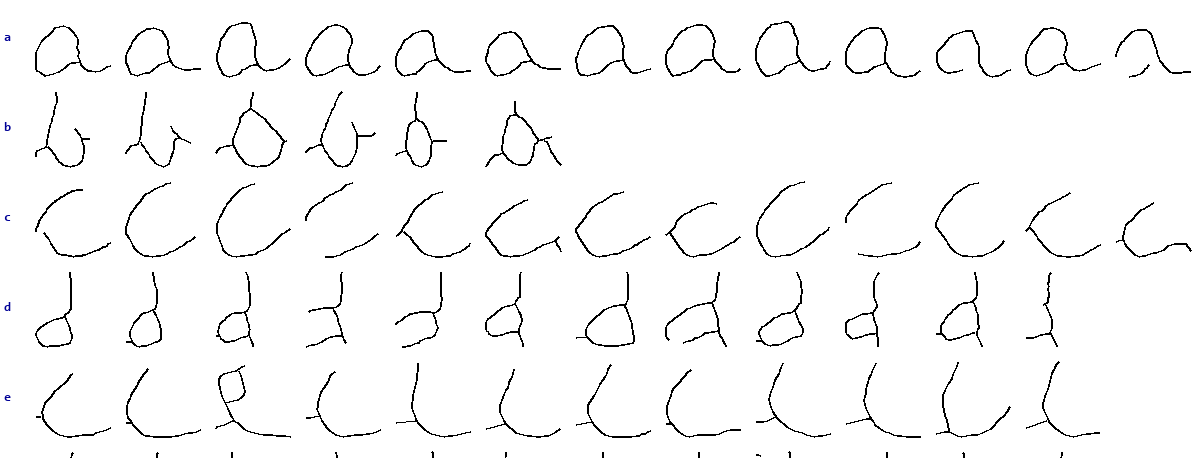
\includegraphics[width=0.78\linewidth]{Figures/w3_glyphs153_ae.png}
\caption{Stored variants of the letters a, b, c, d and e of writer 153, a strongly joined hand; each row is one character with up to 12 variants, the short tails at the sides being remains of ligatures.}
\label{fig:sty-glyphs}
\end{figure}

\subsubsection{Style statistics and permanent storage}
\label{sec:sty-stats}

Besides glyphs, the profile holds measured numbers: slant, pixel x-height, ascender and descender reach, word gap, and \emph{connectedness}, the fraction of adjacent letter pairs whose connection flag was set during tracing. Table~\ref{tab:sty-writers} shows the diversity this is built to reproduce --- slant $-10.5^\circ$ to $42.0^\circ$, connectedness 0.195 to 0.968, word gap 0.94 to 2.68 x-heights across the thirteen writers --- which is requirement R1's diversity target, and the thirteen files (about 4.8\,MB total) load when the server starts.

\begin{table}[!htbp]
\centering
\fontsize{7.5}{9}\selectfont
\setlength{\tabcolsep}{2.5pt}
\begin{tabular}{|l|r|r|r|r|r|r|r|}
\hline
\textbf{Writer} & \textbf{Lines} & \textbf{Slant ($^\circ$)} & \textbf{$x_h$ (px)} & \textbf{$A$} & \textbf{$D$} & \textbf{Gap} & \textbf{Conn.} \\
\hline
150 & 61 & $-4.5$ & 47 & 1.58 & $-0.72$ & 1.33 & 0.343 \\
151 & 58 & 33.0 & 22 & 2.69 & $-1.09$ & 1.59 & 0.968 \\
153 & 66 & 30.0 & 33 & 1.59 & $-1.10$ & 1.59 & 0.961 \\
384 & 54 & 4.5 & 43 & 1.93 & $-0.71$ & 1.37 & 0.500 \\
552 & 47 & $-10.5$ & 32 & 1.62 & $-0.56$ & 1.53 & 0.609 \\
dylan & 79 & $-6.0$ & 26 & 1.68 & $-0.62$ & 1.79 & 0.195 \\
thiya & 48 & 30.75 & 15 & 2.24 & $-1.00$ & 1.65 & 0.962 \\
yeukita & 74 & 0.0 & 27 & 1.45 & $-0.58$ & 0.94 & 0.417 \\
\hline
\end{tabular}
\caption{Representative rows of the thirteen stored style profiles (full table, Appendix~\ref{sec:app-syn}): kept lines, slant, pixel x-height, ascender $A$, descender $D$, word gap in x-heights, and connectedness.}
\label{tab:sty-writers}
\end{table}

\begin{figure}[htb]
\centering
\fbox{\parbox[c][4cm]{0.75\linewidth}{\centering [PLACEHOLDER --- scatter or bar plot of connectedness vs.\ reproduced character accuracy across the thirteen writers]}}
\captionsetup{singlelinecheck=false,justification=justified}
\caption{Placeholder: connectedness (Table~\ref{tab:sty-writers}) plotted against each writer's reproduced character accuracy from Table~\ref{tab:syn-evid}, to show quantitatively that the most joined hands are the hardest to reproduce.}
\label{fig:sty-conn-fig}
\end{figure}

\mustdo{\emph{The builder's \texttt{ExtractLineGlyphs} currently raises an import error} (a stale reference to a function moved during the restructuring of \texttt{TrainText.py}), so no new writer can presently be added and none of the thirteen stored profiles can be regenerated from the page images; the stored profiles themselves are unaffected and still load correctly. \texttt{legibilityLambda} is also absent from all thirteen stored files, so the system synthesises every writer at $\lambda=0$ until the tuner is re-run (Section~\ref{sec:syn-limits}).}

\subsubsection{Synthesis: choosing and placing a glyph}
\label{sec:syn-glyph}
\label{sec:syn-place}

The synthesiser takes text, a style profile, a pen size $x_{\mathrm{mm}}$ in millimetres and a random seed, and returns a \emph{trajectory}, pen-down polylines in millimetres; geometry stays in x-height units until one multiplication at the end, so one profile serves any pen size. Requirement R1 pulls in two directions at once: handwriting that resembles the writer argues for always using the writer's own letters, while handwriting that can be read argues for replacing the writer's worst letters with something clearer. The parameter $\lambda\in[0,1]$ is the single control that sets where a writer sits between those two. The obvious way to trade them off, blending the writer's glyph and a clear \emph{anchor} glyph geometrically, is \emph{not} used, because an average of two different pen strokes is usually not a valid letter at all; instead $\lambda$ scales the \emph{probability} that a chosen variant is replaced by the anchor outright, so every letter drawn is always a real letterform.

Global shear, join probability and line pitch follow from the profile (Equation~\ref{eq:syn-global}); among a writer's own variants for one character the choice is weighted by rank and, when joining, by how well the variant's entry height matches where the pen already is; the anchor-substitution probability is Equation~\ref{eq:syn-swap}; and placement is Equation~\ref{eq:syn-place-eq}:
\begin{align}
\theta_{\mathrm{cap}}&=45^\circ-19^\circ\lambda,\quad\sigma=\tan\!\bigl(\operatorname{clip}(\theta_{\mathrm p},\pm\theta_{\mathrm{cap}})\bigr)+\Delta_\sigma,\quad p_{\mathrm j}=\min(c,1),\label{eq:syn-global}\\
P_{\mathrm{swap}}(\lambda,d)&=\begin{cases}1&d\ge0.55,\\0&\lambda\le10^{-3},\\0.06\,\lambda&d\le0.12,\\\operatorname{clip}\bigl(\lambda\,(0.55+0.9\,b),0,1\bigr),\ b=\operatorname{clip}\bigl(\tfrac{d-0.12}{0.43},0,1\bigr)&\text{otherwise,}\end{cases}\label{eq:syn-swap}\\
X&=P_x+(\ell+x+\sigma_g\,y)\,x_{\mathrm{mm}},\qquad Y=P_y+(y+\delta_g)\,x_{\mathrm{mm}}.\label{eq:syn-place-eq}
\end{align}
A variant beyond prior distance $d=0.55$ is replaced \emph{unconditionally}, whatever $\lambda$; one closer than $d=0.12$ is kept almost always; between those the probability rises with both $d$ and $\lambda$. Below $\lambda=10^{-3}$ substitution switches off entirely, so a writer tuned to zero keeps even their marginal letters. When a writer's medoid itself is too malformed to serve as the anchor, a hand-designed single-stroke skeleton (joined cursive or upright print, re-proportioned to that writer's ascender and descender reach) is used instead, reading back at about 96\,\% character and 84\,\% word accuracy, which is what makes it a usable floor.

Treating connectedness $c$ as a hard threshold, joining every pair above it, was tried first and fused whole words into unbroken blobs, losing the irregularity that makes a hand look human; it is used as a per-pair \emph{probability} $p_{\mathrm j}$ instead. Measured over a design-stage probe, the anchor share this produces ran from 0\,\% for writer 552 to 76\,\% for writer 151, the most joined hand of the set. One pseudo-random stream seeded by the seed argument supplies every draw, so the arguments fix the output completely; at the jitter amplitude the search uses, a letter is perturbed by about a $1.1^\circ$ rotation, a 2.5\,\% scale change and under 0.05\,mm translation. \emph{Style calibration}: because glyphs are placed one instance at a time, an assembled line does not automatically reproduce the writer's own line-level slant and ascender reach (writer 150's ascenders came out about 7\,\% too tall, writer 551's slant about $9^\circ$ too steep against real lines), so a fixed probe sentence is synthesised once per writer and three fixed-point iterations of Equation~\ref{eq:syn-cal} adjust the shear shift $\Delta_\sigma$ and the scale factors $K_A$, $K_D$ until the probe matches the stored real-line reference values:
\begin{equation}
\Delta_\sigma\leftarrow\Delta_\sigma+\tan\theta_{\mathrm{ref}}-\tan\theta_{\mathrm{got}},\quad K_A\leftarrow\operatorname{clip}\Bigl(K_A\frac{A_{\mathrm{ref}}-1}{A_{\mathrm{got}}-1},0.5,1.6\Bigr),\quad K_D\leftarrow\operatorname{clip}\Bigl(K_D\frac{D_{\mathrm{ref}}}{D_{\mathrm{got}}},0.5,1.6\Bigr),
\label{eq:syn-cal}
\end{equation}
with ``ref'' the stored real-line value and ``got'' the probe's measured value by the estimators of Section~\ref{sec:sty-trace}, each correction clipped to bound its effect.

\begin{figure}[htb]
\centering
\fbox{\parbox[c][4.5cm]{0.85\linewidth}{\centering [PLACEHOLDER --- the same letter drawn at $\lambda=0$, $\lambda=0.5$ and $\lambda=1$ for one strongly joined writer, each candidate's prior distance $d$ and swap probability printed beside it]}}
\captionsetup{singlelinecheck=false,justification=justified}
\caption{Placeholder: the legibility sweep of Equation~\ref{eq:syn-swap} on one writer's worst-scoring letter, from the writer's own glyph through partial anchor substitution to the full anchor, with $P_{\mathrm{swap}}$ plotted against prior distance $d$ for several $\lambda$ as an inset curve.}
\label{fig:syn-swap-fig}
\end{figure}

\subsubsection{Best-of-$N$ search with joint scoring}
\label{sec:syn-search}

Single draws vary in quality, so a line is drawn $N$ times and the best kept; the score must use both judges together, because selecting by text accuracy alone raised legibility but lowered writer identification for some writers in a design-stage probe, since the most legible of several random draws need not be the most characteristic.

For a rendered candidate $I$, with $\hat y(I)$ the recogniser's greedy reading and $y$ the intended text, the text term $a(I)$ below is built from the Levenshtein edit distance~\cite{levenshtein1966}, the smallest number of insertions, deletions and substitutions turning one string into the other,
\begin{equation}
a(I)=\max\Bigl(0,1-\frac{\mathrm{Lev}(\hat y(I),y)}{|y|}\Bigr),\quad w(I)=\mathrm{softmax}\bigl(f_{\mathrm{wid}}(I)\bigr)_{a^\star},\quad S(I)=\frac{2\,a(I)\,w(I)}{a(I)+w(I)},
\label{eq:syn-score}
\end{equation}
the harmonic mean of recogniser accuracy and shape-classifier confidence in the target writer $a^\star$, dominated by whichever is smaller, so a candidate cannot win on one criterion while failing the other.

The search has two loops (Figure~\ref{fig:syn-search}): the first draws up to $N$ candidates and keeps the best by $S$; the second, a \emph{repair} loop of at most three rounds, forced-aligns the intended text to the best image, pins the two worst-scoring characters to the anchor, re-synthesises the whole line, and accepts the result only if $S$ strictly improves, so a repair that fixes a letter but makes the line resemble another writer is rejected. $N$ is 6 as the function default, 14 for design-stage measurements, 20 as the web default and 30 in the evaluation script; the cost is entirely judge-bound, synthesising a candidate costing 11 to 16\,ms against 0.5 to 4\,s to score it, so $N$ rather than the construction itself sets the reproduction time of requirement R3.

\begin{figure}[!htbp]
\centering
\begin{tikzpicture}[node distance=3.2mm and 6mm]
\node[w3io] (in) {text, profile, writer $a^\star$, seed base, $N$};
\node[w3box,below=of in] (syn) {synthesise candidate $k$, score by Equation~\ref{eq:syn-score}};
\node[w3dec,below=4.5mm of syn] (loop) {best reaches 0.99,\\or $k=N-1$?};
\node[w3box,below=of loop] (align) {repair: align, pin two weakest\\characters to anchor, re-synthesise};
\node[w3io,below=of align] (out) {best trajectory (at most 3 repair rounds)};
\draw[w3arr] (in) -- (syn);
\draw[w3arr] (syn) -- (loop);
\draw[w3arr] (loop.west) -- node[w3lab,above,pos=0.3]{no} ++(-14mm,0) |- (syn.west);
\draw[w3arr] (loop) -- node[w3lab,right]{yes} (align);
\draw[w3arr] (align) -- (out);
\end{tikzpicture}
\caption{Control flow of the candidate search of \texttt{SynthesizeJointBestOf}, simplified from the full state machine; both the main loop and the repair loop use the joint score of Equation~\ref{eq:syn-score}.}
\label{fig:syn-search}
\end{figure}

Table~\ref{tab:syn-evid} lists the measurements that motivated the design, over six novel sentences, two seeds and ten writers. Joint best-of-$N$ at $N=14$ reached 97.5 / 95.8\,\% writer identification and 81.6 / 81.4\,\% character accuracy (direct / through G-code); on a matching comparison of identical words, synthesis costs 7.4 percentage points of character accuracy against the writers' own real handwriting (89.0\,\% vs.\ 81.6\,\%) and more than 1.5 times the word accuracy (70.5\,\% vs.\ 46.7\,\%), which locates the loss in spacing and word boundaries rather than in letterforms.

\begin{table}[!htbp]
\centering
\fontsize{8}{9.6}\selectfont
\setlength{\tabcolsep}{4pt}
\begin{tabularx}{\linewidth}{|X|c|c|}
\hline
\textbf{Stage} & \textbf{Writer ID, direct / G-code (\%)} & \textbf{Char.\ acc., direct / G-code (\%)} \\
\hline
Plain synthesis after label and glyph fixes & 79.2 / 80.0 & 75.9 / 76.3 \\
Text-only best-of-$N$ with plain repair & 76.7 / 73.3 & 83.8 / 82.7 \\
Joint best-of-$N$, $N=14$ & 97.5 / 95.8 & 81.6 / 81.4 \\
\hline
Final system, 13 writers, 3 sentences, $N=8$ & 92.3 / 89.7 & 79.2 / 79.2 \\
\hline
Matching comparison: writers' own real handwriting & not applicable & 89.0 / --- \\
Matching comparison: synthesis of the same words & not applicable & 81.6 / --- \\
\hline
\end{tabularx}
\caption{Measurements that motivated the design (upper block) and the final system (lower blocks). Only the two matching-comparison rows are independent of the search and so the figures to trust most directly; the rest are qualified by Section~\ref{sec:syn-limits}.}
\label{tab:syn-evid}
\end{table}

\begin{figure}[!htbp]
\centering

\includegraphics[width=0.95\linewidth]{Figures/w3_synth_150.png}\\[1pt]
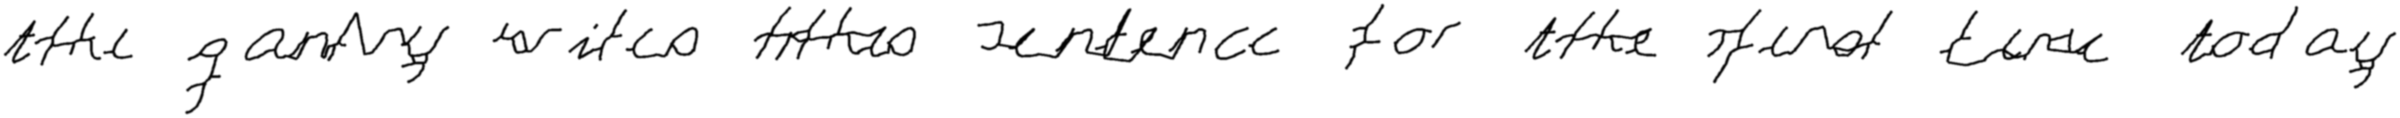
\includegraphics[width=0.95\linewidth]{Figures/w3_synth_153.png}
\caption{Synthesised line for writer 150 (upper, printed hand, read back with three small errors) and writer 153 (lower, joined hand, read back with several letter errors), one seed and candidate each, rendered from an end-to-end run.}
\label{fig:syn-lines}
\end{figure}

\subsubsection{Alternatives considered}

A recurrent sequence generator with attention and a mixture-density stroke output, the approach that first generated convincing on-line handwriting from a recurrent network~\cite{graves2013}, needs hundreds to thousands of lines of on-line pen data per writer, where only 47 to 130 scanned lines exist per writer here; a from-scratch version trained on skeleton-derived strokes learned slant, roundness and connectedness but no legible letters, and was rejected. Adversarial and diffusion generators conditioned on a style exemplar~\cite{kang2020,dai2024} need less data through pre-training but emit a raster needing the same thinning to vectorise, cannot control size, slant and spacing as explicit numbers, and took 35 to 45\,s per line in a trial against 3 to 8\,s for glyph synthesis, so they were parked. The approach closest in spirit to the one built here is exemplar-based synthesis from a writer's own captured letterforms~\cite{haines2016}, re-assembling stored shapes rather than generating pixels from a learned distribution; the glyph library needs about nine pages per writer and no training, exposes every parameter as an explicit number, and costs about 15\,ms per candidate, which suits a single-board computer with no accelerator; its one clear weakness is joined hands, whose joins are necessarily lost by the character-cutting of Section~\ref{sec:sty-forced}.

\subsubsection{Known faults and limitations}
\label{sec:syn-limits}

\begin{enumerate}\setlength{\itemsep}{0pt}\setlength{\parskip}{0pt}
\item \emph{The legibility mechanism is inert as submitted}, because \texttt{legibilityLambda} is absent from all thirteen stored profiles and defaults to zero, so $\lambda=0$ on the live path: only the unconditional substitutions at $d\ge0.55$ fire, and every $\lambda$-dependent figure above describes a tuned configuration that is not what the delivered profiles currently run.
\item Every figure after the search is introduced is the opinion of the very networks that selected the output: the search loads the same weight files as the measurement, so the values show the pipeline can satisfy its two judges, not that an independent reader would agree.
\item $\lambda$, the anchor threshold and $N$ were tuned on the same sentences Section~\ref{sec:results} measures, and the style calibration of Section~\ref{sec:syn-glyph} measures both sides with the same estimator, so its agreement is partly self-fulfilling.
\item Writers 151 and 552, the two most joined hands, reach only 53 and 56\,\% character accuracy through G-code against about 84\,\% for the other eleven, the clearest limitation of the exemplar approach and a direct consequence of the cutting problem of Section~\ref{sec:sty-forced}.
\item Cutting a joined line destroys how a letter changes shape with its neighbours, which is the underlying reason writers 151 and 551 are reproduced least legibly.
\end{enumerate}
